\documentclass{article}
\usepackage[x11names]{xcolor}
\usepackage{pgfplots}
\usepgfplotslibrary{fillbetween}

\begin{document}

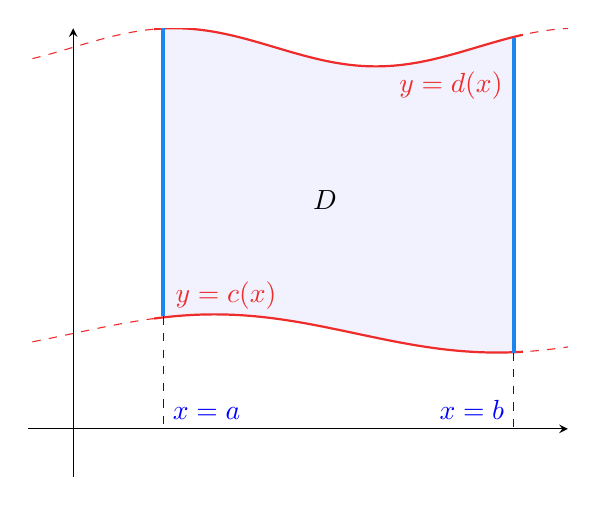
\begin{tikzpicture}
\begin{axis}[xmin=-0.5, ymin=-0.5, xmax=5.5, axis lines=middle, ticks=none]

\addplot[dashed, Firebrick2, samples=1000, domain=-1:0.9]{sin(deg(x))/5+1};
\addplot[name path=g2, thick, Firebrick2, samples=1000, domain=0.9:5]{sin(deg(x))/5+1}node at (axis cs:1.7,1.4) {$y=c(x)$};
\addplot[dashed, Firebrick2, samples=1000, domain=4.9:5.5]{sin(deg(x))/5+1};

\addplot[dashed, Firebrick2, samples=1000, domain=-1:0.9]{sin(deg(1.4*x))/5+4};
\addplot[name path=g1, thick, Firebrick2, samples=1000, domain=0.9:5]{sin(deg(1.4*x))/5+4}node[] at (axis cs:4.2,3.6){$y=d(x)$};
\addplot[dashed, Firebrick2, samples=1000, domain=4.9:5.5]{sin(deg(1.4*x))/5+4};


\addplot[DodgerBlue2,mark=none, ultra thick] coordinates {(1, 4.2) (1, 1.18)};
\addplot[DodgerBlue2,mark=none, ultra thick] coordinates {(4.9, 0.8)(4.9, 4.1)};

\addplot +[blue,mark=none, dashed]coordinates {(1, 1.18) (1, 0)}node[anchor=south west] {$x=a$};
\addplot +[blue,mark=none, dashed]coordinates {(4.9, 0.8) (4.9, 0)}node[anchor=south east] {$x=b$};

\node at (axis cs:2.8,2.4) {$D$};

\addplot [
        thick,
        color=blue,
        fill=blue, 
        fill opacity=0.05,
    ]
fill between[
        of=g1 and g2,
        soft clip={domain=1:4.9},
    ];
\end{axis}
\end{tikzpicture}

\end{document}